%%% Choose between 16:9 and 4:3 format by commenting out/uncommenting one of the following lines:
\documentclass[aspectratio=169]{beamer} % 16:9
% \documentclass{beamer} % 4:3

%=========================================================================================================================

\usepackage[english]{babel}     % English language
\usepackage[latin1]{inputenc}   % Input encoding
\usepackage{tikz}               % For creating graphics
\usepackage{subfig}
\usepackage[mode=buildnew]{standalone}
\usepackage{url}                % For including urls
\usepackage{tabularx}           % For better tables
\usepackage{xcolor}             % Für bunte Farbe :)

\usetheme{aig}                  % Set beamer theme

%=========================================================================================================================
\title{Qualit\"at von Wikipedia-Artikeln}

\author[]{Alexander Kunze, Sebastian Bunge, Johannes Kr\"amer, Emmanuelle Steenhof, Robin Suxdorf}
\institute{Artificial Intelligence Group,\\
University of Hagen, Germany}
\date{\today}
%=========================================================================================================================
\logo{
\includegraphics[width=3cm]{figures/logoaig.png}}
%=========================================================================================================================

\begin{document}

%=========================================================================================================================

% frame
% block
% alertblock
% exampleblock

% \highlight{}
% \darkhighlight{}
% \yellowhighlight{}
% \mathhighlight{}
% \darkmathhighlight{}
% \yellowmathhighlight{}

% appendix

\begin{frame}
    \titlepage
\end{frame}
\nologo

\begin{frame}{Problemstellung}
    \begin{figure}
        \centering
        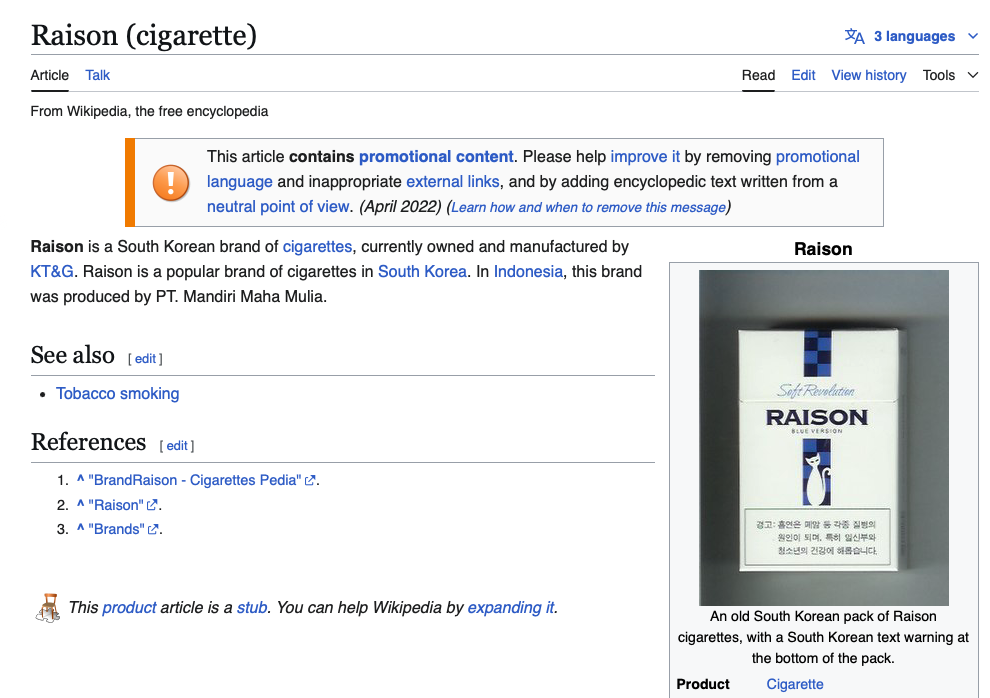
\includegraphics[width=0.6\linewidth]{figures/example_promo_article.png}
        \caption{\url{https://en.wikipedia.org/wiki/Raison\_(cigarette)}}
        \label{fig:enter-label}
    \end{figure}
\end{frame}

\begin{frame}{Problemstellung}
    \begin{block}{Wann ist ein Wikipedia-Artikel gut?}
        \begin{itemize}
            \item redaktionelle Standards (Good article Kriterien)
            \begin{itemize}
                \item gut geschrieben
            
                \item korrekte und \"uberpr\"ufbare Informationen

                \item neutral in der Sichtweise

                \item verwenden Bilder mit geeigneten Urheberrechtslizenzen
            \end{itemize}

            \item Good article nomination (GAN)

            \pause

            \item nur 0.59\% der Wikipedia-Artikel sind gut (1 von 171)
        \end{itemize}
    \end{block}

    \pause

    \begin{block}{Problemstellung}
        Ist ein gegebener Wikipedia-Artikeln gut oder promotional? \\

        Zusatz: Falls ein Wikipedia-Artikel nicht gut ist, warum?
    \end{block}
\end{frame}

\section{Daten}

\begin{frame}{Daten}
    \begin{figure}
        \centering
        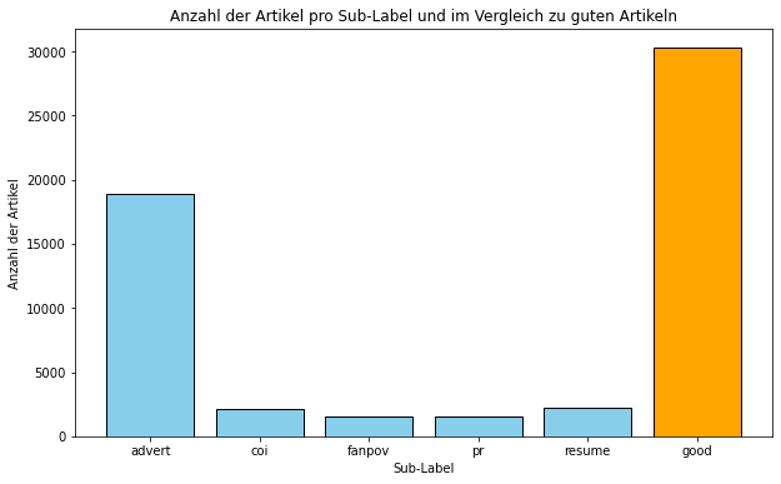
\includegraphics[width=0.8\linewidth]{figures/distribution_multiple_classes.png}
    \end{figure}
\end{frame}

\subsection{Datenvorverarbeitung}

\begin{frame}{Datenvorverarbeitung}
    \begin{block}{Datenvorverarbeitung}
        \begin{itemize}
            \item Entfernung von Sonderzeichen und Kleinbuchstabierung

            \item Entfernung von f\"uhrenden und folgenden Leerzeichen

            \item Optional Stopw\"orter und Zahlen entfernen

            \item Textrepr\"asentation mittels TF-IDF-Vektorisierung:
                  \begin{itemize}
                      \item Maximale Anzahl von Features
                      \item n-Gramm-Bereich
                      \item Minimale Dokumentenfrequenz (\texttt{min\_df})
                      \item Maximale Dokumentenfrequenz (\texttt{max\_df})
                  \end{itemize}
        \end{itemize}
    \end{block}
\end{frame}

\section{Ans\"atze}

\begin{frame}{Genereller Ansatz}
    \begin{block}{Genereller Ansatz}
        \begin{itemize}
            \item Metriken
            \begin{itemize}
                \item Precision

                \item Recall
    
                \item $F_1$-Score
            \end{itemize}

            \item One-vs-Rest Strategie

            \item Hyperparameteroptimierung durch GridSearch
        \end{itemize}
    \end{block}
\end{frame}

\subsection{Logistische Regression}

\begin{frame}{Logistische Regression (1)}
    \begin{block}{Hyperparameter}             
        \begin{itemize}
            \item Regularisierungsparameter \(C\): \{0.01, 0.1, 1, 10, 100\}
            
            \item Verschiedene Solver (\texttt{lbfgs}, \texttt{saga})

            \item Strafterm: \(L1\) oder \(L2\)-Regularisierung
            
            \item Maximale Anzahl von Features: \{5000, 10000, 20000\}
            
            \item n-Gramm-Bereich: \{(1,1), (1,2), \dots ,(3,4)\}
        \end{itemize}
    \end{block}
\end{frame}

\begin{frame}{Logistische Regression (2)}
    \begin{block}{Ergebnisse}
        \begin{figure}
            \centering
            
            \subfloat {{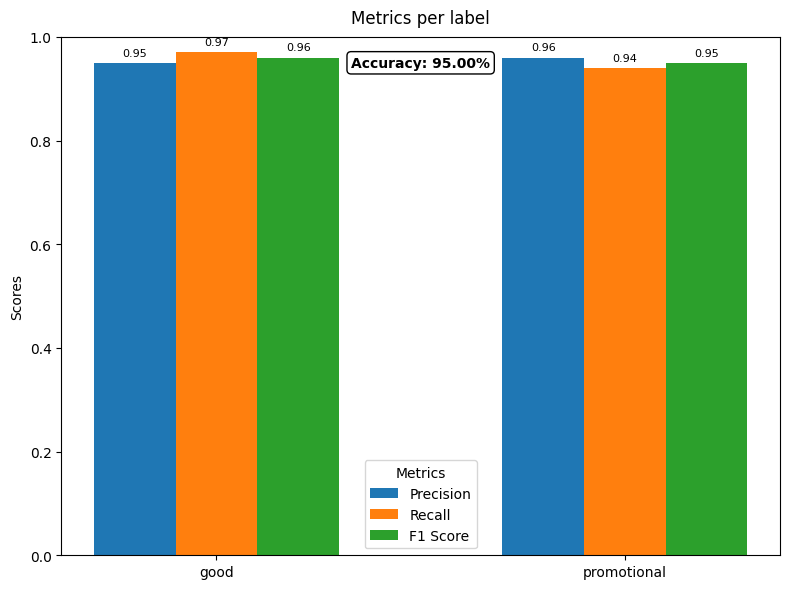
\includegraphics[width=.4\textwidth, height=5cm]{figures/evaluation_log_reg_b.png}}}
            \qquad
            \subfloat {{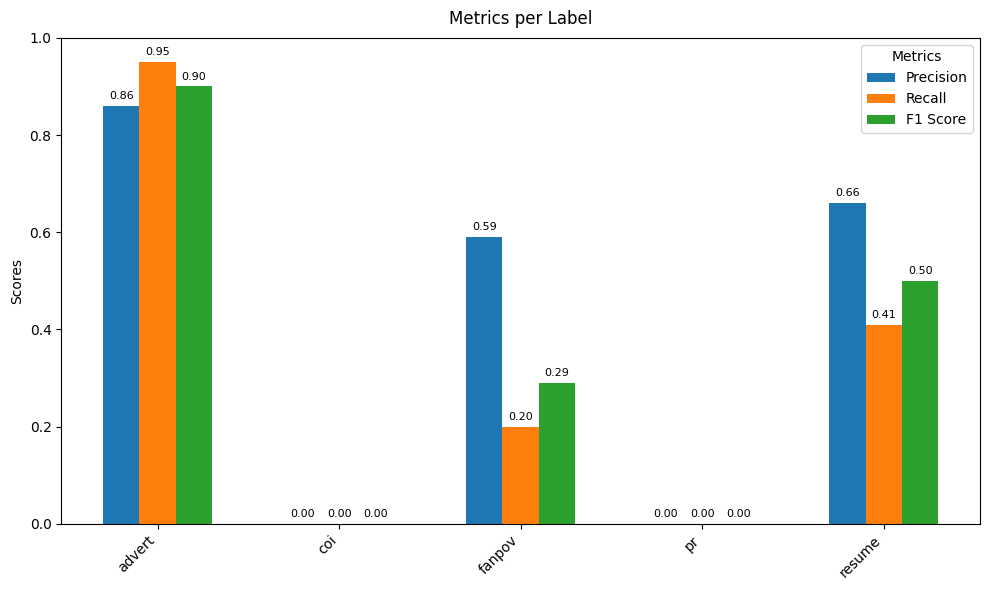
\includegraphics[width=.4\textwidth, height=5cm]{figures/evaluation_log_reg_m.png}}}
        \end{figure}
    \end{block}
\end{frame}

\subsection{Support Vector Machine}

\begin{frame}{Support Vector Machine (1)}
    \begin{block}{Hyperparameter}
        \begin{itemize}
            \item Vergleich verschiedener Kernels:
                \begin{itemize}
                    \item \texttt{linear}, \texttt{poly}, \texttt{rbf}, \texttt{sigmoid}
                    
                    \item Keine Vorteile gegen\"uber \texttt{linear} festzustellen
                \end{itemize}

            \item Regularisierungsparameter
        \end{itemize}
    \end{block}
\end{frame}

\begin{frame}{Support Vector Machine (2)}
    \begin{block}{Ergebnisse}
        \begin{figure}
            \centering
            
            \subfloat {{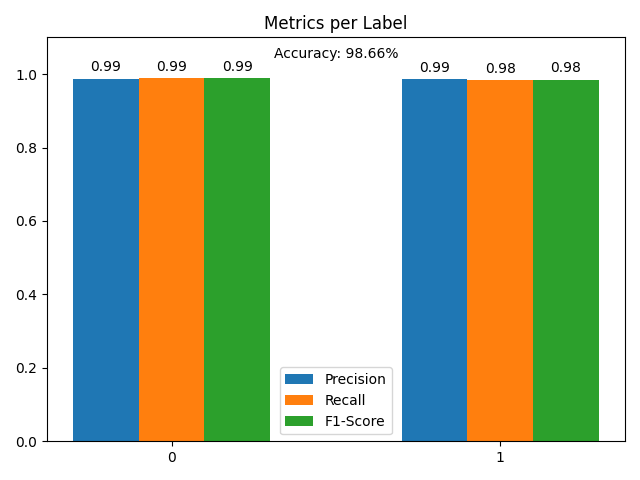
\includegraphics[width=.4\textwidth, height=5cm]{figures/evaluation_linear_svm.png}}}
            \qquad
            %\subfloat {{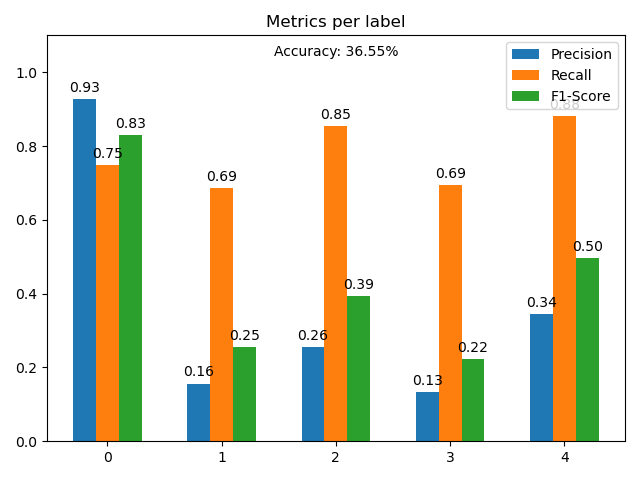
\includegraphics[width=.4\textwidth, height=5cm]{figures/evaluation_nbm.png}}}
        \end{figure}
    \end{block}
\end{frame}

\subsection{Bayes Klassifikator}

\begin{frame}{Bayes Klassifikator (1)}
    \begin{block}{Gew\"ahlte Hyperparameter}
        \begin{itemize}
            \item Textrepr\"asentation mittels TF-IDF-Vektorisierung:
                  \begin{itemize}
                      \item Maximale Anzahl von Features: 10.000
                      
                      \item n-Gramm-Bereich: Unigramme (1,1)
                      
                      \item Minimale Dokumentenfrequenz (\texttt{min\_df}): 0.001
                      
                      \item Maximale Dokumentenfrequenz (\texttt{max\_df}): 0.9
                  \end{itemize}
                  
            \item Einstellung des Gl\"attungsparameters \(\alpha = 1.0\)
        \end{itemize}
    \end{block}
\end{frame}

\begin{frame}{Bayes Klassifikator (2)}
    \begin{block}{Ergebnisse}
        \begin{figure}
            \centering
            
            \subfloat {{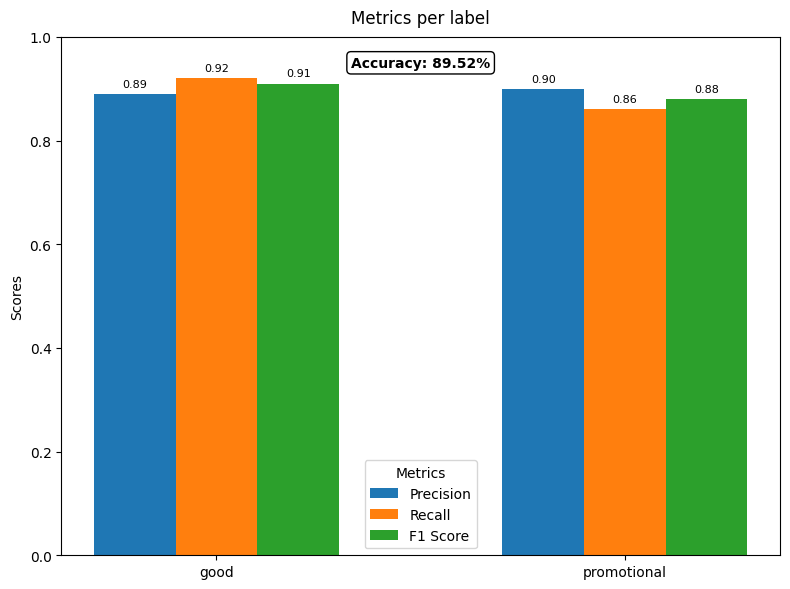
\includegraphics[width=.4\textwidth, height=5cm]{figures/evaluation_nbb.png}}}
            \qquad
            \subfloat {{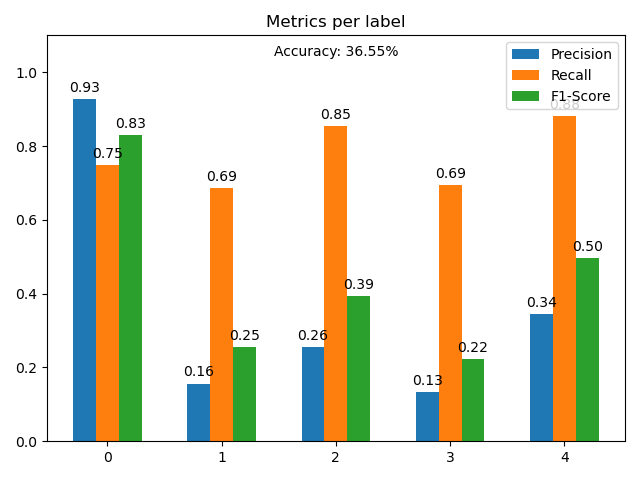
\includegraphics[width=.4\textwidth, height=5cm]{figures/evaluation_nbm.png}}}
        \end{figure}
    \end{block}
\end{frame}

\subsection{Convolutional Neural Network}

\begin{frame}{Convolutional Neural Network (1)}
    \begin{block}{Datenvorverarbeitung}
        \begin{itemize}
            \item Textrepr\"asentation mittels Byte Pair Encoding (\texttt{cl100k\_base})

            \item Einheitliche Textl\"ange: gegebenenfalls Padtokens erg\"anzen

            \item Embedding Layer: ein Embeddingvektor pro Token
        \end{itemize}
    \end{block}

    \pause

    \begin{block}{Hyperparameter}
        \begin{itemize}
            \item Modellparameter (Auswahl)
            \begin{itemize}
                \item Tokenizer, Embedding Dimension

                \item Anzahl Faltungs-Layer, Filtergr\"o{\ss}en

                \item Feed Forward Neural Network
            \end{itemize}

            \item Trainingsparameter
            \begin{itemize}
                \item Learning Rate

                \item Batch Size

                \item Anzahl Epochen
            \end{itemize}
        \end{itemize}
    \end{block}
\end{frame}

\begin{frame}{Convolutional Neural Network (2)}
    \begin{block}{Ergebnisse}
        \begin{figure}
            \centering
            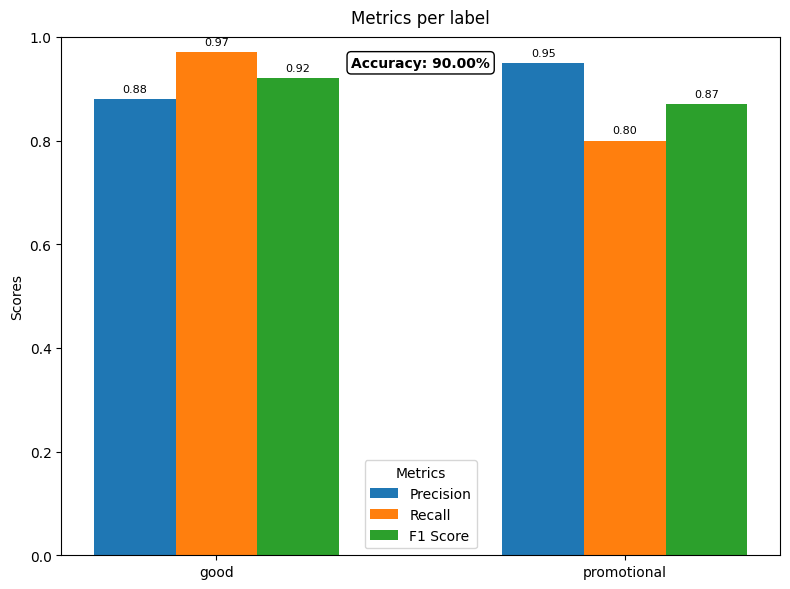
\includegraphics[width=6.8cm]{figures/evaluation_cnnb.png} 
        \end{figure} 
    \end{block}
\end{frame}

\section{Zusammenfassung und Ausblick}
\begin{frame}
    \begin{block}{Zusammenfassung und Ausblick}
        \begin{itemize}
            \item Gemachte Arbeit
            \begin{itemize}
                \item Drei klassische und ein Deep Learning Verfahren implementiert
                
                \item F\"unfter Ansatz: erste Ideen gesammelt und Experimente gemacht
            \end{itemize}

            \pause
            
            \item Problem: ungleiche Verteilung der Label

            \pause
        
            \item N\"achste Schritte
            \begin{itemize}
                \item Datensatz erweitern
                \begin{itemize}
                    \item Wikipedia-Dump
                    
                    \item Datenaugmentation (Synonyme ersetzen, \"Ubersetzungen, LLMs)
                    
                    \item Transfer Learning (wissenschaftliche Paper)
                \end{itemize}
    
                \item Hyperparameter-Optimierung
    
                \item Vortrainierte Modelle verwenden
            \end{itemize}
        \end{itemize}
    \end{block}

    \pause

    Vielen Dank!
\end{frame}
\end{document}
